Als erster Schritt wurden einige Fakten und Rahmenbedingungen zum Projekt ausgelegt und so das Umsystem definiert.
\begin{itemize}
	\item Die Grundmotivation Projekts ist hauptsächlich ästhetischer Natur.
	\item Es bietet (voraussichtlich) weder marktwirtschaftlicher noch funktionellen Nutzen.
	\item Es besteht auch kein Auftraggeber- oder Kundenverhältnis in dem Sinne, und somit auch keine damit verknüpften Interessen.
	\item Markteinführung nicht zwingend, daher auch keine Zielgruppen bzw. Benutzer per se.
	\item Es liegt in dem Sinne auch kein systematisches Problem vor, welches gelöst werden soll.
	\item Das Projekt soll innerhalb von 14 Wochen realisiert werden.
	\item Es wurden bereits einige Vorarbeiten als Vorleistung getätigt (siehe \ref{vorarbeiten}).
	\item Zum Zeitpunkt der Arbeit sind aufwändige physikalische Simulationsprogramme wie COMSOL o.ä. nicht oder nur beschränkt verfügbar.
	\item Zudem war kein Zugang zu einer anechoischen Kammer verfügbar, worin z.B. die Abstrahlcharakteristik sehr genau hätte gemessen werden können.
	\item Als Produktionsstandort stand das FabLab Winterthur zur Verfügung.
	\item Die Firma \href{https://www.joyned.at/}{JOYNED GmbH} \begin{minipage}{3cm}
		\vspace{-1mm}
		
\includegraphics[scale=1.5]{pictures/joyned_logo.png}
	\end{minipage} erklärte sich bereit, ihr Fachwissen und Beratung zur Implementierung ihrer MILAN-Software zur Verfügung zu stellen.
\end{itemize}
\subsection{SWOT Analyse}
Anhand der gegebenen Aufgabenstellung wurde nun eine SWOT-Analyse durchgeführt, in der die Ausgangslage nach Stärken (\textit{strenghts}), Schwächen (\textit{weaknesses}), Chancen (\textit{opportunities}) und Gefahren (\textit{threats}) kategorisiert wurde. Diese sind in Abbildung \ref{pics:swot}  abgebildet und zeigten deutlich, das die Ausgangslage geprägt ist von Schwächen, jedoch für die Zukunft überwiegen Chancen bereitstellt. Die der Ist-Zustand konnte somit als \textit{High Risk - High Reward} Situation bezeichnet werden.
\begin{figure}[H]
	\centering
	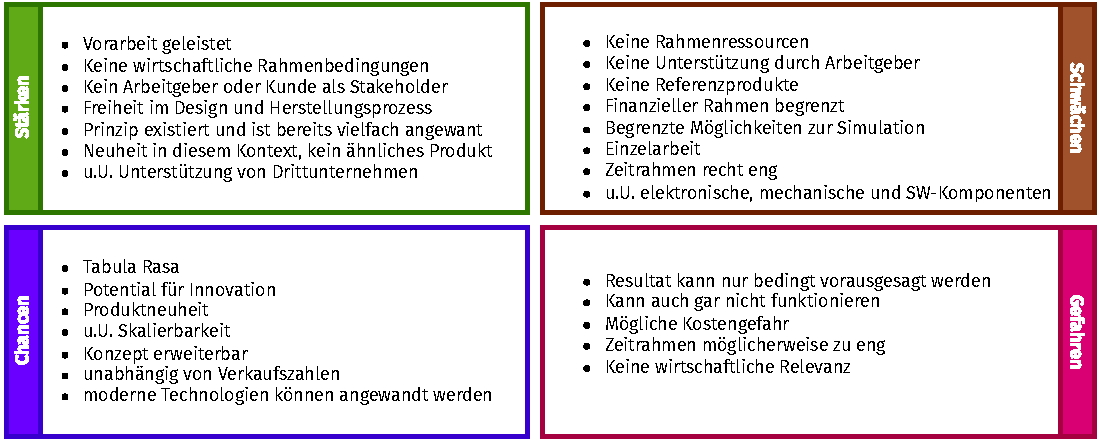
\includegraphics[width=\textwidth]{pictures/SWOT.pdf}
	\caption{SWOT-Analyse}
	\label{pics:swot}
\end{figure}
\subsection{Ishikawa Diagramm}
Die möglichen Problemursachen für das Projekt wurden nun kategorisiert und danach in Abbildung \ref{pics:ishikawa} aufgezeichnet. Es zeigte sich, dass sich die (möglichen) Problemursachen in folgende Oberkategorien aufteilen liessen:
\paragraph{Physik} Hier ist zum einen das grundlegende Phänomen, welches genutzt werden soll recht komplex und von vielen Faktoren abhängig. Zum anderen muss eine Saite in Schwingung versetzt werden, was physikalisch gesehen nicht unbedingt eine Effiziente Methode zur Klangerzeugung ist.
\paragraph{Material} Nebst den Faktoren wie Materialdichte, Gewicht und Nachgiebigkeit\footnote{siehe: \href{https://de.wikipedia.org/wiki/Compliance_(Physiologie)}{Compliance (Physiologie)}}, spielte vor allem auch die Herstellungsmöglichkeiten eine Rolle: Wie kann ein Material in welchen Dimensionen produziert werden?
\paragraph{Engineering} Hier ist vor allem die Hardware- und Software zu nennen. Je nach Variante können dabei keines, eines oder beide obsolet werden. Zudem können aus der Signalübertragung her auch Fehlerquellen entstehen.
\paragraph{Zeit} Der Zeitfaktor gilt wohl als grösster Problemverursacher, da der Abgabetermin fix vorgegeben ist und nicht verschoben werden kann.
\paragraph{Budget} Da kein Auftraggeber oder Firma als finanzielle Unterstützung vorhanden ist, muss das ganze Projekt aus privaten Reserven finanziert werden.
\paragraph{Produktesicherheit} Obwohl das Produkt nicht direkt als Verkaufsprodukt vorgesehen ist, muss die Sicherheit doch als Faktor miteinbezogen werden.
\vspace{6mm}
\begin{figure}[H]
	\centering
	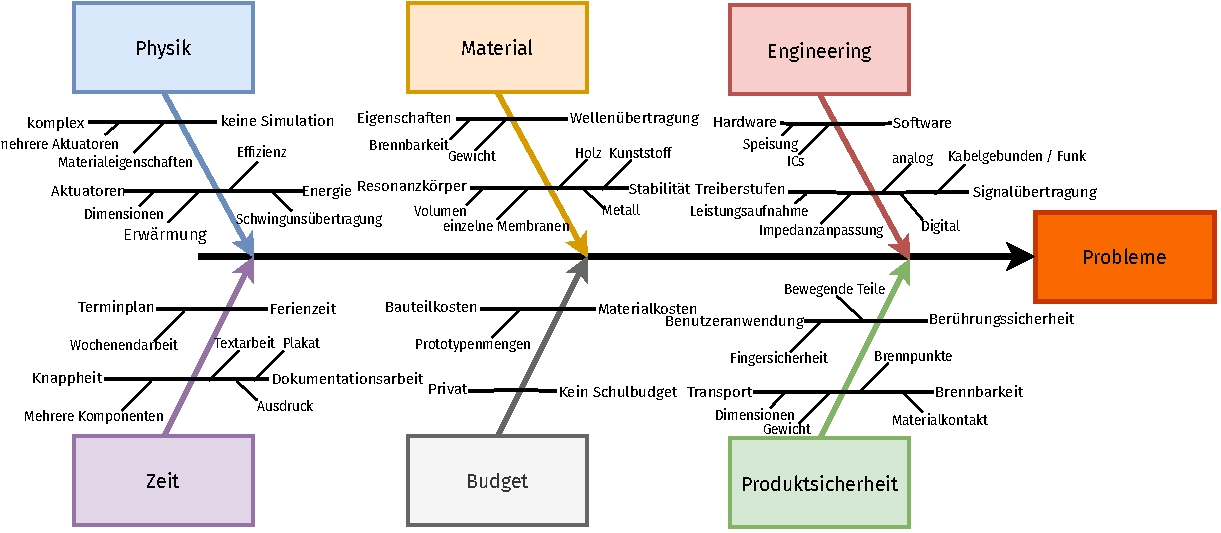
\includegraphics[width=\textwidth]{pictures/ishikawa.pdf}
	\caption{Ishikawa-Analyse}
	\label{pics:ishikawa}
\end{figure}